\documentclass[10pt]{beamer}

\usetheme{metropolis}
\usepackage{appendixnumberbeamer}

\usepackage{booktabs}
\usepackage{multirow}
\usepackage[scale=2]{ccicons}

\usepackage{pgfplots}
\usepgfplotslibrary{dateplot}

\usepackage{xspace}
\usepackage{xcolor}
\newcommand{\themename}{\textbf{\textsc{metropolis}}\xspace}
\usepackage{tabularx}

\usepackage[utf8]{inputenc}
\usepackage[brazilian]{babel}

\usepackage{blindtext}
\usepackage[portuguese, noend, plain, linesnumbered]{algorithm2e}

\setbeamercolor{background canvas}{bg=white}

\title{}
\subtitle{Uso de Redes de Função de Base Radial e Cadeias de Markov para detecção online de mudanças de conceito em fluxos contínuos de dados}
\date{}
\author{\textbf{Discente:} Ruivaldo Neto \newline \textbf{Orientador:} Ricardo Rios}
\institute{Universidade Federal da Bahia \newline Departamento de Ciência da Computação \newline Programa de Pós-Graduação em Ciência da Computação \newline\newline Contato: rneto@rneto.dev \newline\newline 04 de Fevereiro de 2020}

\titlegraphic{%
  \begin{picture}(0,0)
    \put(330, 28){\makebox(0,0)[rt]{
\includegraphics[scale=0.25]{logo.png}}}
  \end{picture}
}

\begin{document}

\maketitle

\begin{frame}{Roteiro}
  \setbeamertemplate{section in toc}[sections numbered]
  \begin{minipage}{\textwidth}
    \tableofcontents
  \end{minipage}
\end{frame}

\section{Concept Drift}

\begin{frame}{Concept Drift}
    \begin{itemize}
        \item<1 -> \alert{Mudanças de conceito} são alterações no contexto do processo e/ou na distribuição dos dados que podem impactar negativamente técnicas de AM.
        \item<1 -> Podem ser definidas formalmente através da Teoria Bayesiana de Decisão \cite{Duda:2000:PC:954544}: sendo $p_{t_0}$ e $p_{t_1}$ as distribuições de probabilidades conjuntas nos instantes $t_0$ e $t_1$, há mudança de conceito entre $t_0$ e $t_1$ se:
        \begin{equation} \label{eq:3}
            {\exists}X : p_{t_0}(X, c) \ne p_{t_1}(X, c)
        \end{equation}
        % \item<1 -> $X$ possui uma classificação legítima em $t_0$, mas passa a ter outra, também legítima, em $t_1$.
    \end{itemize}
\end{frame}

\begin{frame}{Mudança de Conceito}
    \begin{itemize}
        \item<1 -> São categorizadas como \alert{Virtuais} ou \alert{Reais} \cite{Gama:2014:SCD:2597757.2523813}:
        \begin{itemize}
        \item<1 -> \alert{Mudanças Virtuais} são alterações na probabilidade a priori das classes, $P(c)$, e \alert{\textbf{não modificam} os resultados esperados}.
        \item<1 -> \alert{Mudanças Reais} são alterações na probabilidade a posteriori, $p(c|X)$, e \alert{\textbf{modificam} os resultados esperados}.
        \end{itemize}
    \end{itemize}
\end{frame}

\begin{frame}{Mudança de Conceito}
\begin{figure}[H]
    \begin{center}
        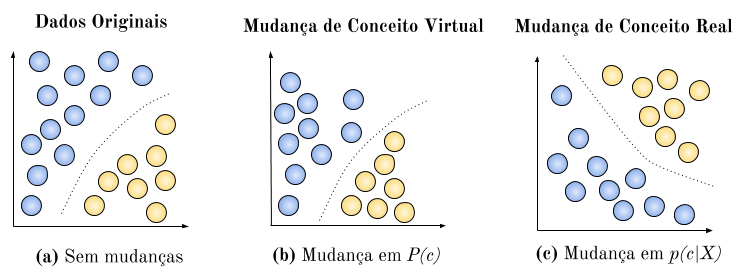
\includegraphics[scale=0.55]{imagens/concept_drift.png}
        \caption{Mudança de Conceito Virtual vs. Mudança de Conceito Real.}
        \label{fig:real_and_virtual_concept_drift}
    \end{center}
\end{figure}
\end{frame}

\begin{frame}{Mudança de Conceito}
    \begin{itemize}
        \item<1 -> Ocorrem de forma \alert{abrupta}, \alert{gradual}, \alert{incremental} ou \alert{recorrente} \cite{Zliobaite:2010}.
    \end{itemize}
    \begin{figure}[H]
        \begin{center}
            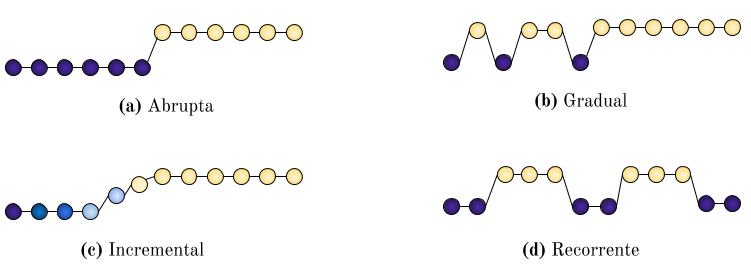
\includegraphics[scale=0.55]{imagens/concept_drift_patterns.png}
            \caption{Padrões de ocorrência de Mudanças de Conceito.}
            \label{fig:concept_drift_patterns}
        \end{center}
    \end{figure}
\end{frame}

\begin{frame}{Algoritmos para Detecção de Mudança de Conceito}
    \begin{itemize}
        \item<1 -> Algoritmos de detecção se dividem em dois grupos, conforme a necessidade de rotulação dos dados \cite{Zliobaite:2010}:
        \begin{itemize}
        \item<1 -> \alert{Explícitos/Supervisionados}: \textbf{Dependem} da rotulação dos dados. Realizam a detecção a partir do monitoramento de medidas de performance como taxa de erro e acurácia.
        \item<1 -> \alert{Implícitos/Não Supervisionados}: \textbf{Independem} da rotulação dos dados. Realizam a detecção através do monitoramento de características dos próprios dados ou de indicadores produzidos pelas técnicas de aprendizado aplicadas.
        \end{itemize}
    \end{itemize}
\end{frame}

\section{RBFChain}

\begin{frame}{Redes de Função de Base Radial}
    \begin{itemize}
        \item<1 -> \alert{Redes de Função de Base Radial} são redes neurais cuja ativação é realizada através do cálculo da distância entre o evento e um centro definido \cite{Braga:RedesNeuraisTeoriaAplicacoes}.
        \item<1 -> A arquitetura mais básica para redes RBF envolve três camadas:
        \begin{itemize}
            \item<1 -> \alert{Entrada}: Recepciona os dados e encaminha para camada intermediária.
            \item<1 -> \alert{Intermediária}: Composta por funções de ativação de base radial que atuam como neurônios.
            \item<1 -> \alert{Saída}: Pondera os resultados da camada intermediária, agregando-os linearmente para compor a resposta final da rede.
        \end{itemize}
        % \item<1 -> Na literatura, as funções Gaussianas são as funções de ativação mais empregadas em redes RBF.
      \end{itemize}
\end{frame}

\begin{frame}{Redes de Função de Base Radial}
    \begin{figure}[H]
    \begin{center}
        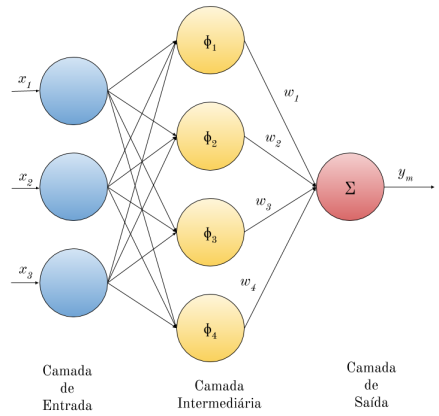
\includegraphics[scale=0.63]{imagens/rbf_arq.png}
        \caption{Arquitetura RBF.}
        \label{fig:rbg_arq}
    \end{center}
    \end{figure}
\end{frame}

\begin{frame}{Redes de Função de Base Radial}
    \begin{itemize}
        \item<1 -> O RBFChain utiliza uma rede RBF adaptada, composta apenas pelas camadas inicial e intermediária.
        \item<1 -> O processo de ativação da camada intermediária produz, implicitamente, grupos dos eventos recebidos.
        \item<1 -> Mudanças de conceito são identificadas quando o grupo ativo desse agrupamento é alterado.
      \end{itemize}
\end{frame}

\begin{frame}{Cadeias de Markov}
    \begin{itemize}
        \item<1 -> \alert{Cadeias de Markov} são processos estocásticos no qual a probabilidade do estado em um determinado período de tempo depende apenas do estado no período imediatamente anterior (Equação \ref{eq:markov}).
        \begin{equation}
            \label{eq:markov}
            \mathbb { P } \left( X _ { t } = s _ { j } | X _ { t - 1 } = s _ { i } , \ldots , X _ { 0 } = s _ { 0 } \right) = \mathbb { P } \left( X _ { t } = s _ { j } | X _ { t - 1 } = s _ { i } \right) = p _ { i j }
        \end{equation}
      \end{itemize}
\end{frame}

\begin{frame}{Cadeias de Markov}
    \begin{itemize}
        \item<1 -> A Cadeia de Markov pode assumir os estados $a_1, a_2, \ldots, a_r$, de tal modo que a probabilidade de transição de um estado $a_i$ para um estado $a_j$ seja $P_{ij}$ (um valor dependente apenas de $i$ e $j$);
        \item<1 -> As probabilidades entre estados podem ser representadas por uma matriz estocástica (Equação \ref{eq:matriz_estocastica}):
        \begin{equation}
            \label{eq:matriz_estocastica}
            P = \left[ \begin{array} { c c c c } { P _ { 11 } } & { P _ { 12 } } & { \dots } & { P _ { 1 r } } \\ { P _ { 21 } } & { P _ { 22 } } & { \dots } & { P _ { 2 r } } \\ { \vdots } & { \vdots } & { \vdots } & { \vdots } \\ { P _ { r 1 } } & { P _ { r 2 } } & { \cdots } & { P _ { r r } } \end{array} \right]
        \end{equation}
      \end{itemize}
\end{frame}

\begin{frame}{Cadeias de Markov}
    \begin{figure}[H]
        \begin{center}
            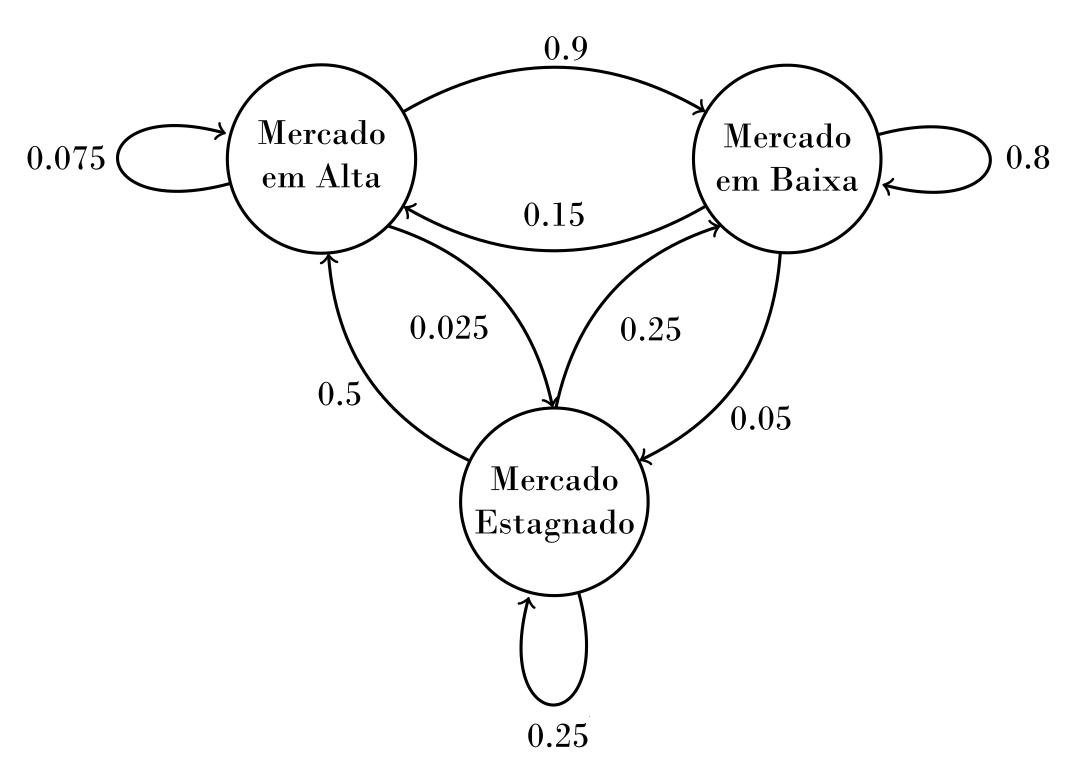
\includegraphics[scale=0.23]{imagens/markov_chain_wikipedia.png}
            \caption{Representação Gráfica: Cadeia de Markov com três estados.}
            \label{fig:cadeia_markov_tres_estados}
        \end{center}
    \end{figure}
\end{frame}

\begin{frame}{Cadeias de Markov}
    \begin{itemize}
        \item<1 -> O RBFChain utiliza uma Cadeia de Markov para modelar o agrupamento criado na rede RBF adaptada.
        \item<1 -> Os grupos formados representam os estados e as ativações de novos grupos, as transições.
        \item<1 -> As transições são refletidas no modelo markoviano através do aumento da probabilidade correspondente e a diminuição proporcional das outras transições, respeitando a condição: $0 \leq P_{ij} \leq 1$.
      \end{itemize}
\end{frame}

\begin{frame}{Visão Geral}
    \begin{itemize}
        \item<1 -> O RBFChain atua diretamente sobre o fluxo de dados e é composto por dois componentes principais: uma Rede de Função de Base Radial (RBF) adaptada e uma Cadeia de Markov.
      \end{itemize}
\end{frame}

\begin{frame}{Visão Geral}
        \begin{figure}[H]
            \begin{center}
                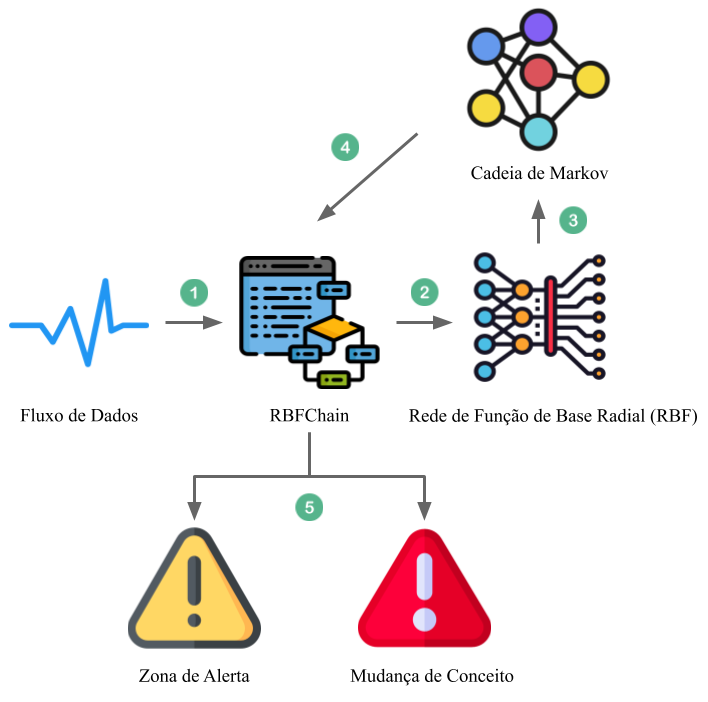
\includegraphics[scale=0.4]{imagens/arquitetura_rbfchain.png}
                \caption{Arquitetura RBFChain.}
                \label{fig:arquitetura}
            \end{center}
        \end{figure}
\end{frame}


\begin{frame}{Execução de exemplo}
    \begin{itemize}
        \item $S = {0.11, 0.12, 0.13, 0.33, 0.34, 0.45, 0.6, 0.33, 0.25, 0.14, 0.11, 0.15}$
        \item $\sigma = 3, \lambda = 0.8, \alpha = 0.25, \delta = 0.5$
    \end{itemize}
    \begin{figure}[H]
        \begin{center}
            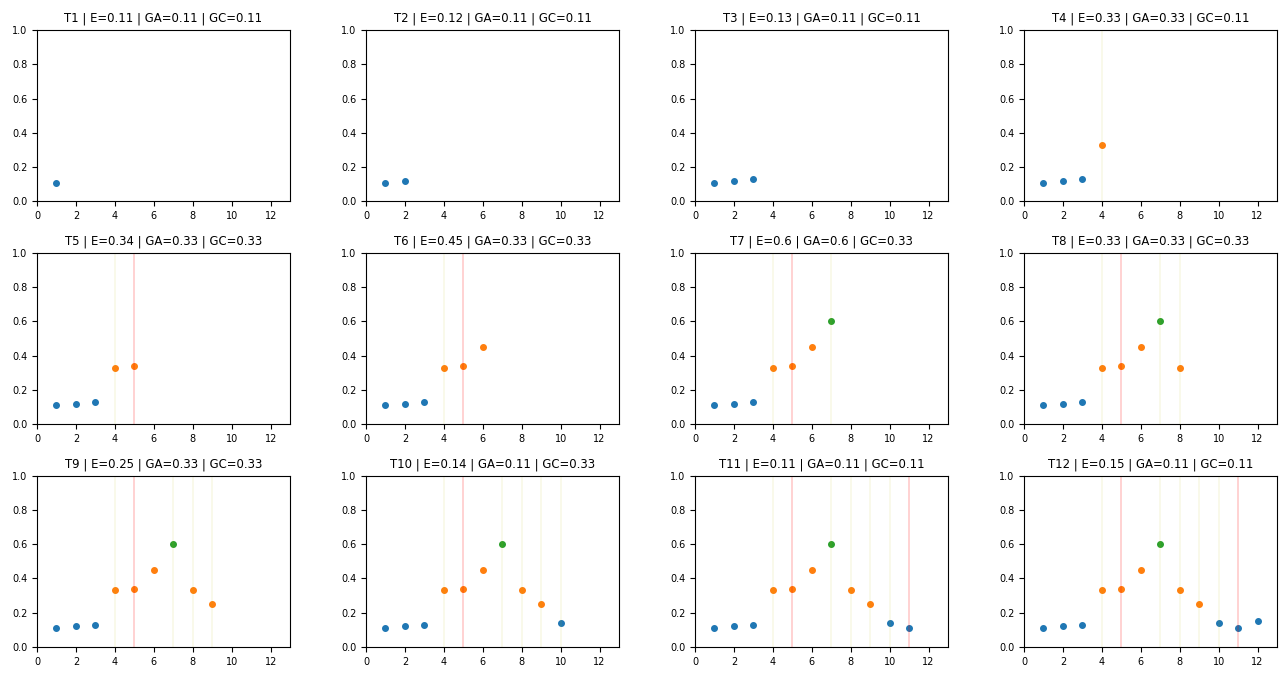
\includegraphics[width=\textwidth]{imagens/funcionamento_algoritmo.png}
            \caption{Execução de exemplo do RBFChain.}
            \label{fig:funcionamento_algoritmo}
        \end{center}
    \end{figure}
\end{frame}

\begin{frame}{Execução de exemplo}
    \begin{figure}[H]
        \begin{center}
            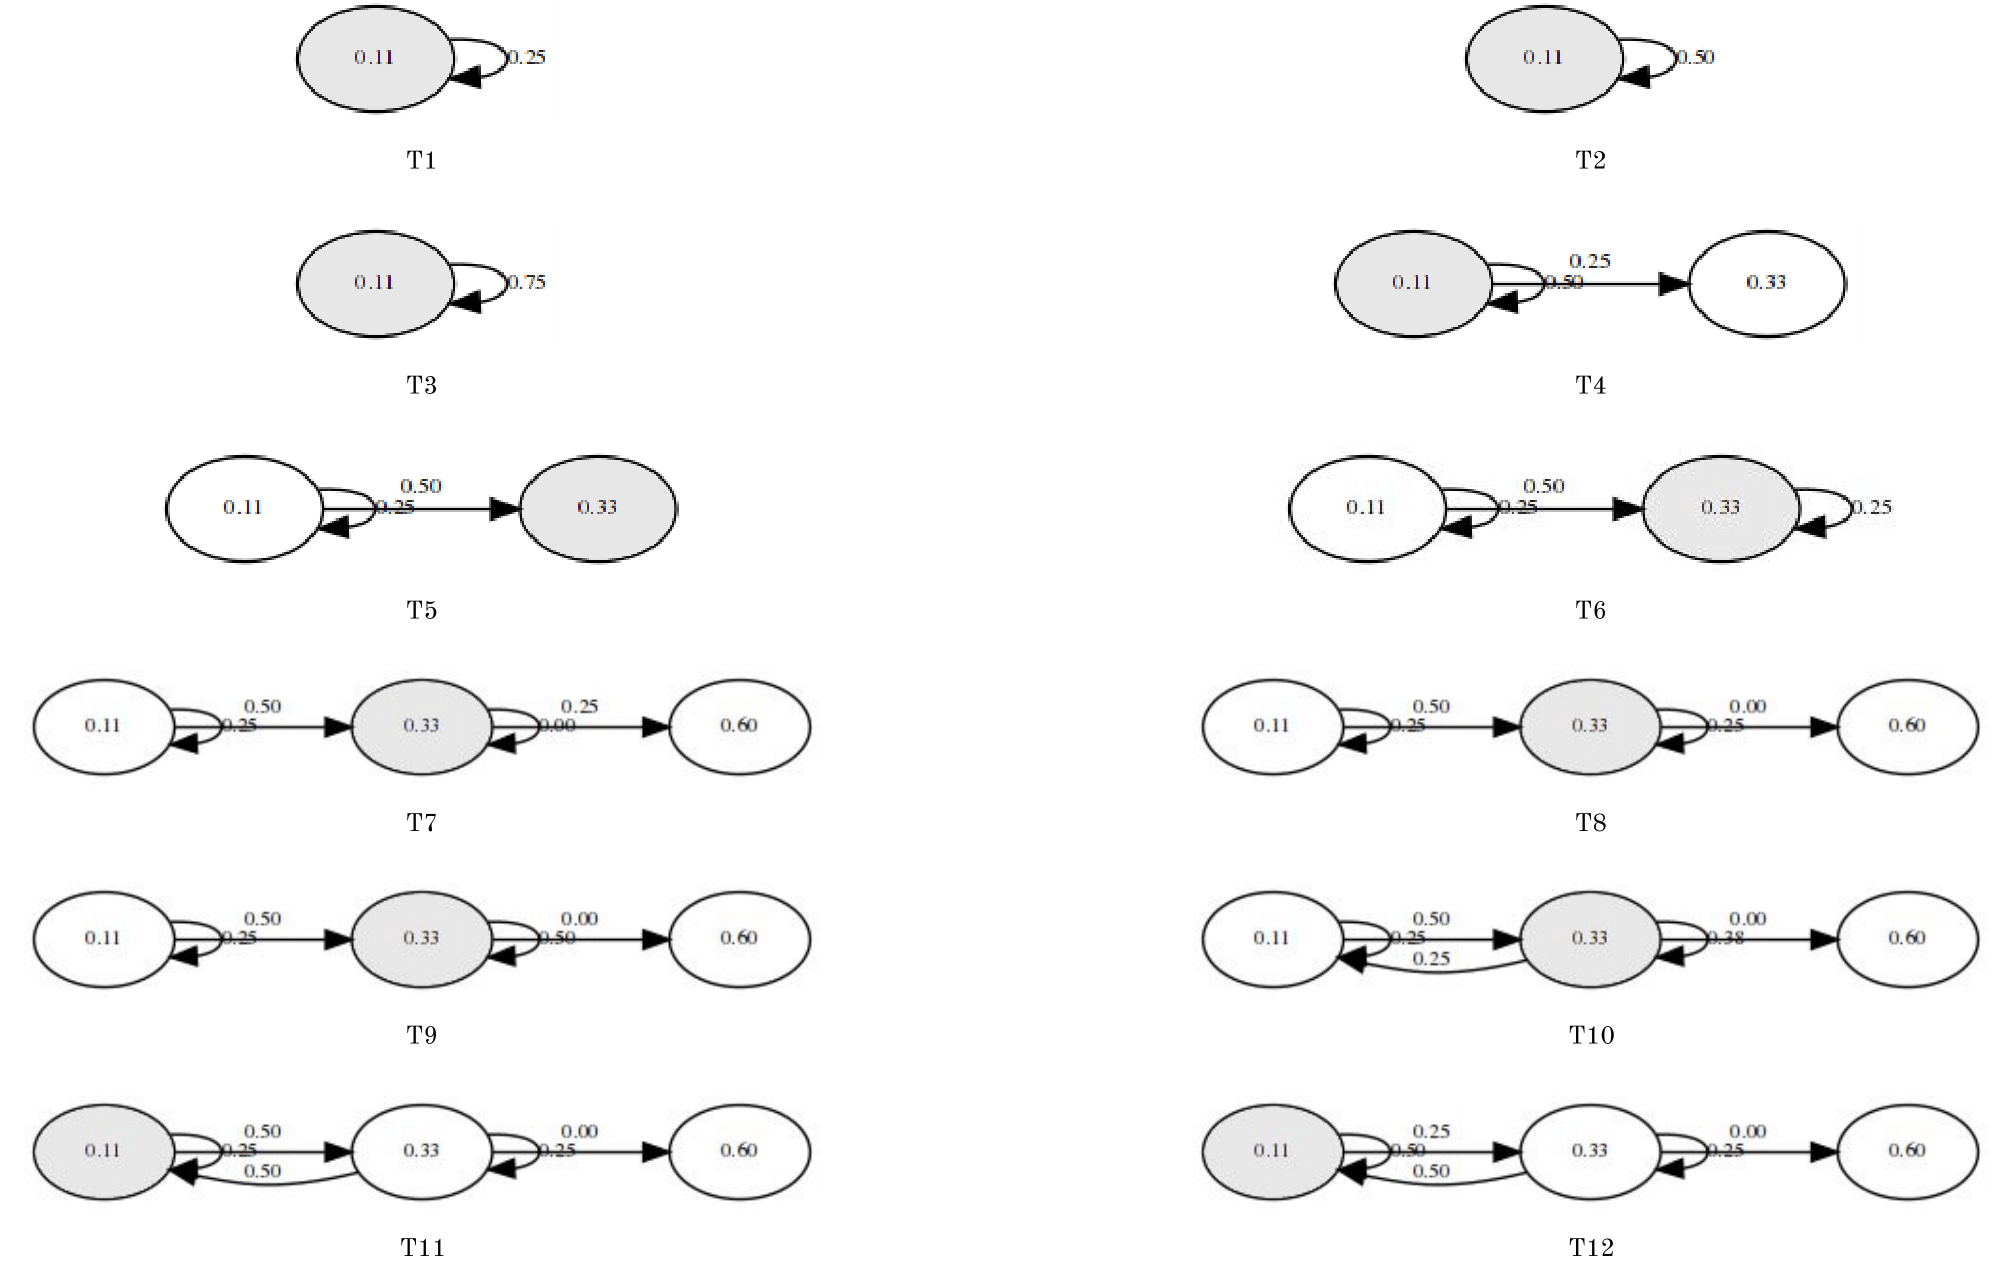
\includegraphics[width=\textwidth]{imagens/evolucao_markov.png}
            \caption{Evolução do modelo markoviano.}
        \label{fig:evolucao_markov}
        \end{center}
    \end{figure}
\end{frame}


\section{Experimentos}

\begin{frame}{Dados Sintéticos}
    \begin{figure}[ht]
        \begin{center}
            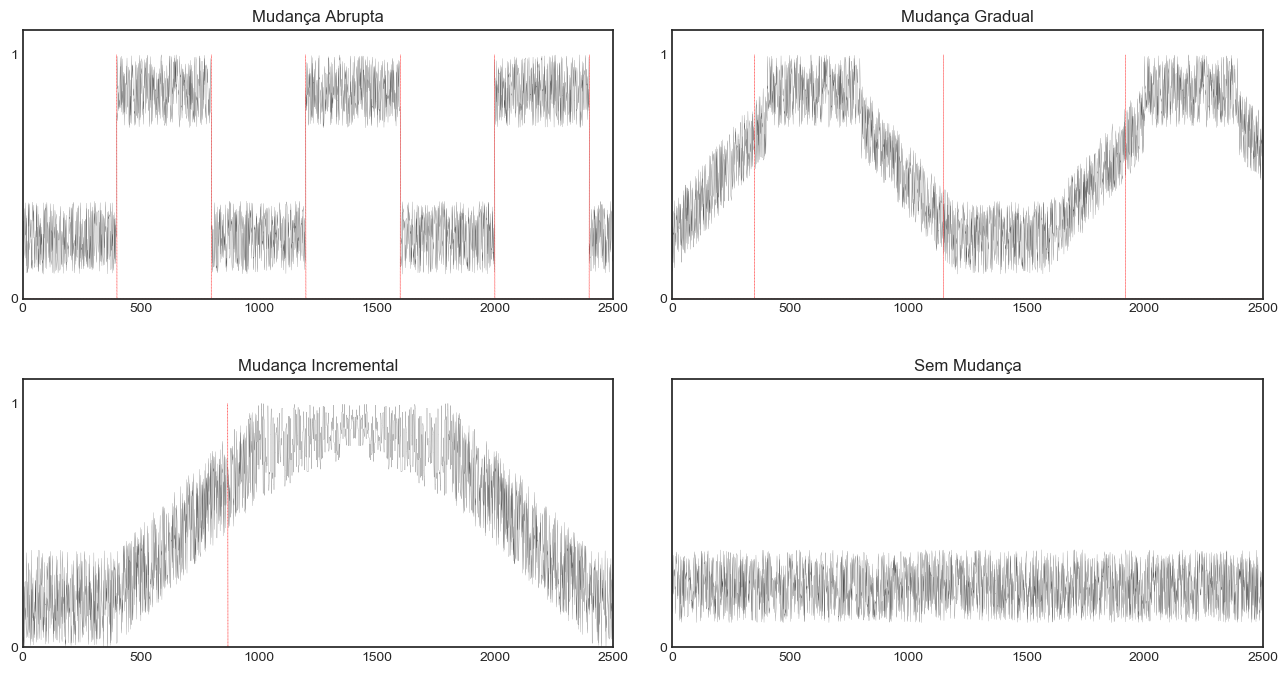
\includegraphics[width=\textwidth]{imagens/conjuntos_dados_sinteticos.png}
            \caption{Representação gráfica dos conjuntos de dados sintéticos.}
            \label{fig:conjuntos_dados_sinteticos}
        \end{center}
    \end{figure}
\end{frame}

\begin{frame}{Dados Sintéticos -  Sem mudanças de conceito}
    \begin{figure}[t]
        \begin{center}
            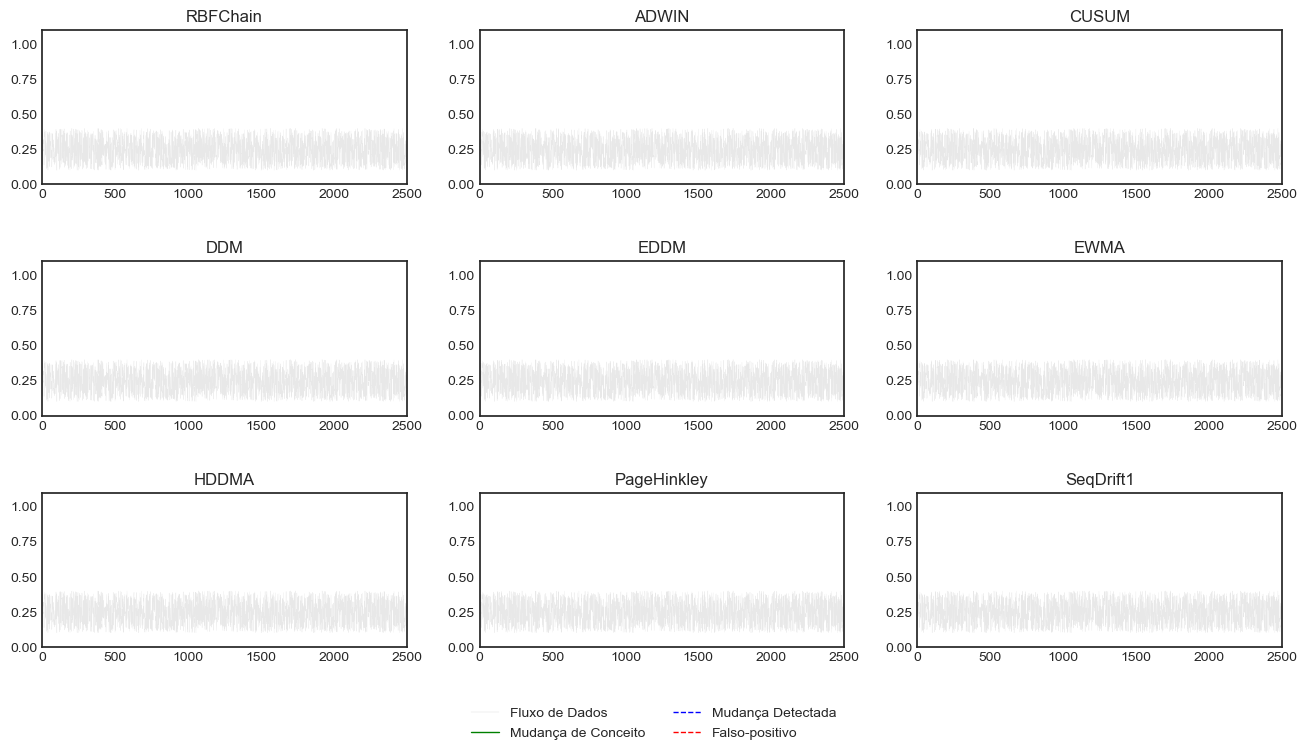
\includegraphics[width=\textwidth]{imagens/nochange.png}
            \caption{Comportamento dos algoritmos para o conjunto de dados sem mudanças de conceito.}
            \label{fig:exp_sem_mudancas}
        \end{center}
    \end{figure}
\end{frame}

\begin{frame}{Dados Sintéticos -  Mudanças Abruptas}
    \begin{figure}[t]
        \begin{center}
            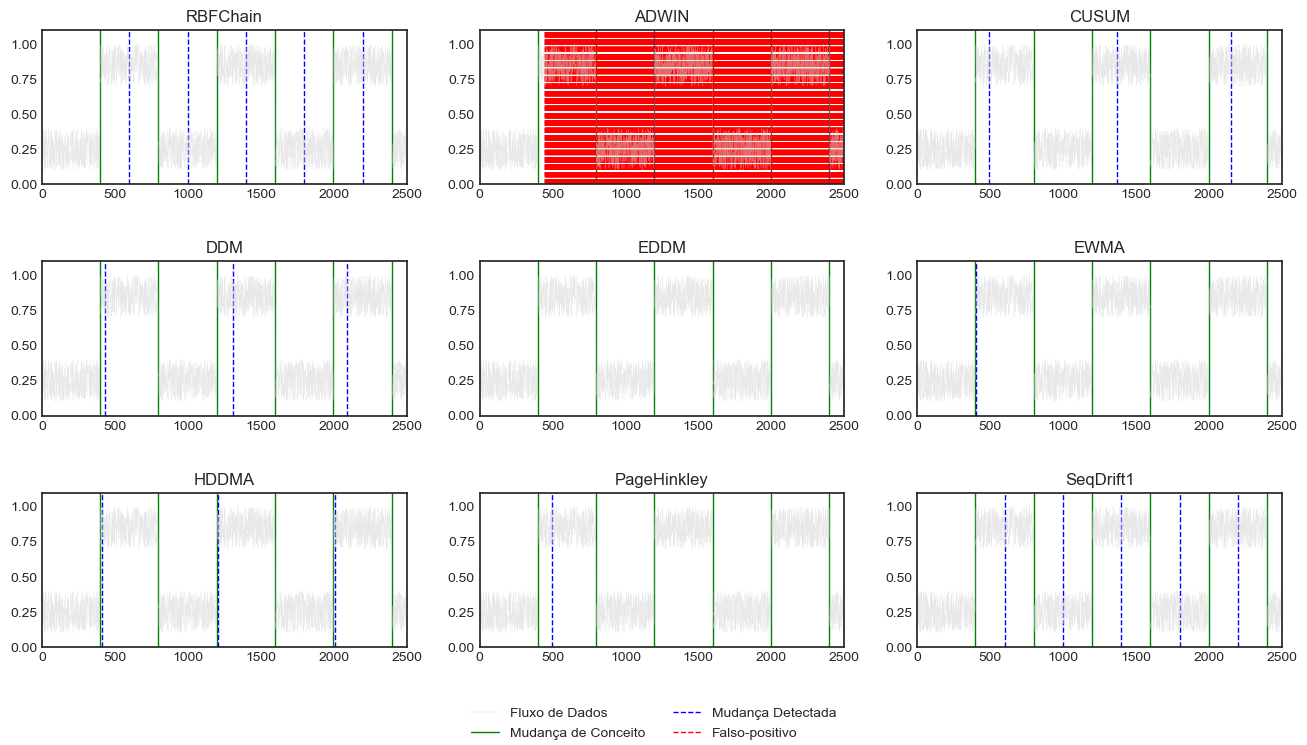
\includegraphics[width=\textwidth]{imagens/abrupt.png}
            \caption{Comportamento dos algoritmos para o conjunto de dados com mudanças de conceito abruptas.}
            \label{fig:exp_abrupta}
        \end{center}
    \end{figure}
\end{frame}

\begin{frame}{Dados Sintéticos -  Mudanças Graduais}
    \begin{figure}[t]
        \begin{center}
            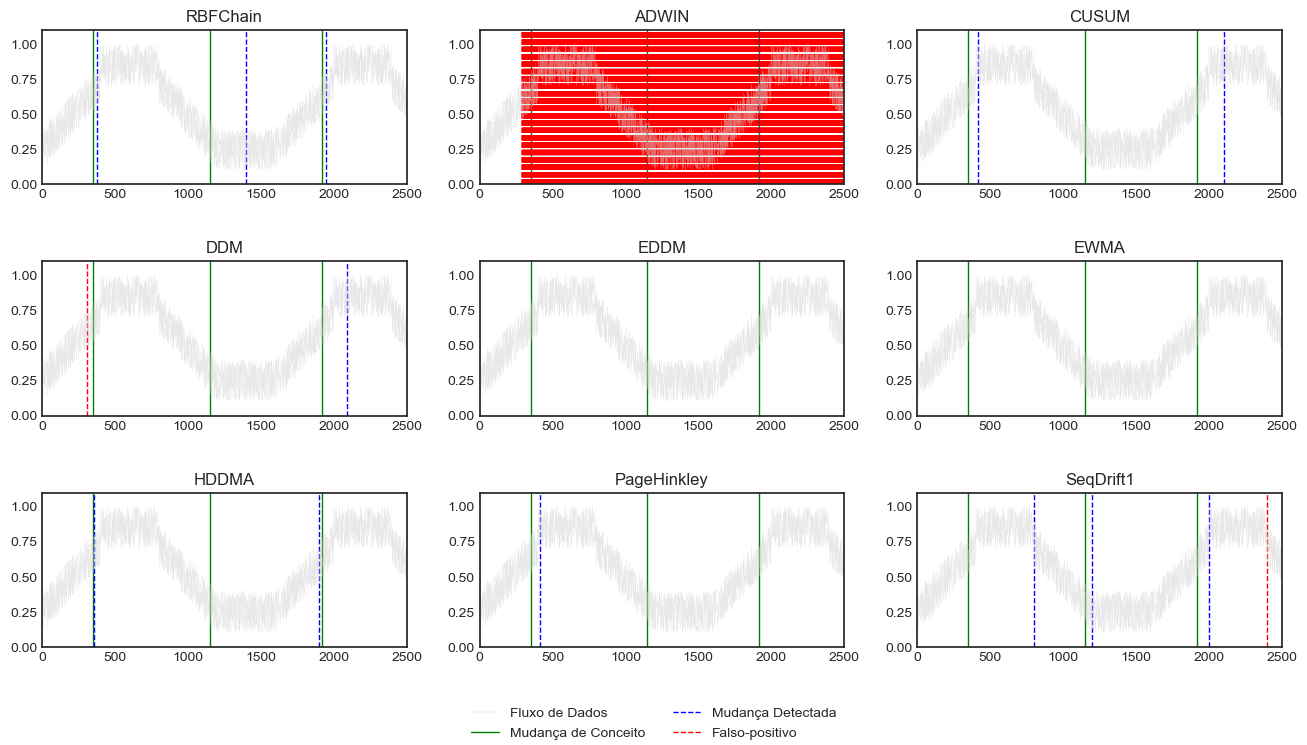
\includegraphics[width=\textwidth]{imagens/gradual.png}
            \caption{Comportamento dos algoritmos para o conjunto de dados com mudanças de conceito graduais.}
            \label{fig:exp_gradual}
        \end{center}
    \end{figure}
\end{frame}

\begin{frame}{Dados Sintéticos -  Mudanças Incrementais}
    \begin{figure}[t]
        \begin{center}
            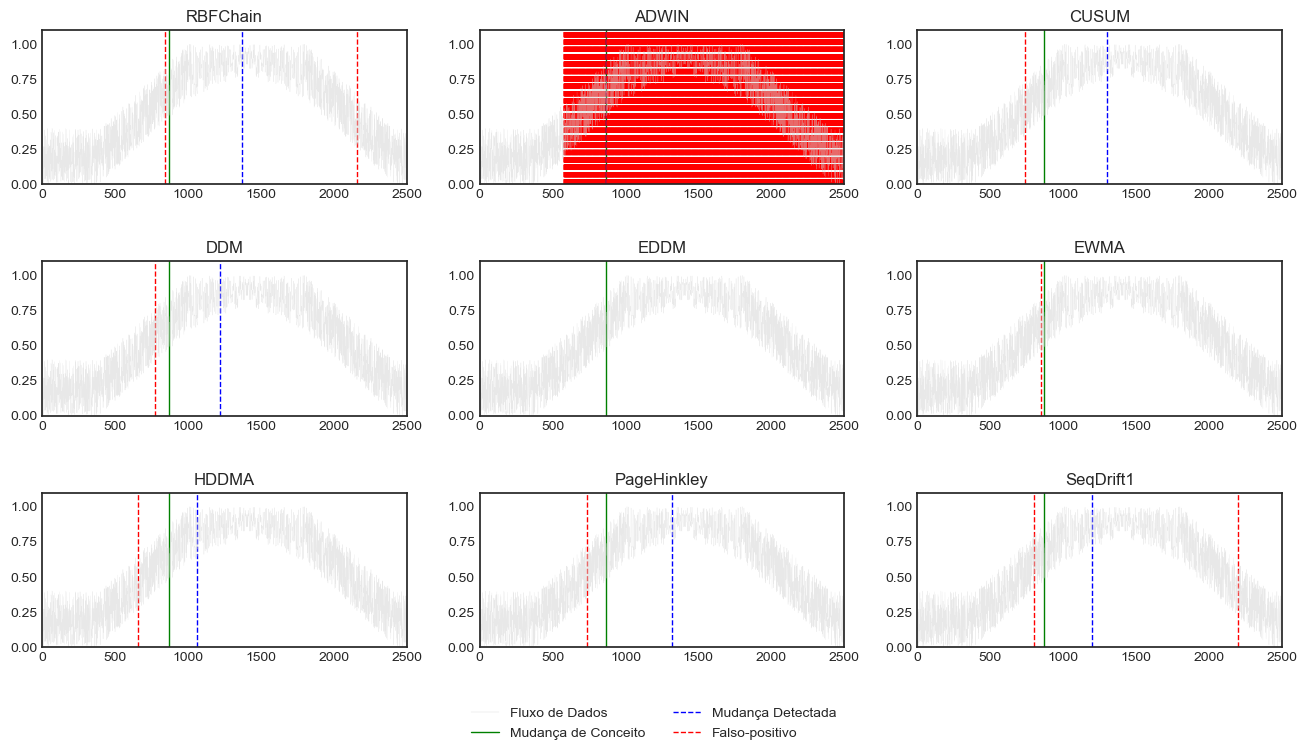
\includegraphics[width=\textwidth]{imagens/incremental.png}
            \caption{Comportamento dos algoritmos para o conjunto de dados com mudanças de conceito incrementais.}
            \label{fig:exp_incremental}
        \end{center}
    \end{figure}
\end{frame}

\begin{frame}{Dados Reais - Identificação de fixações e sacadas}
    \begin{itemize}
        \item O experimento utilizou dados de dois macacos-prego (Dede e Juju) produzidos e cedidos pelo Instituto do Cérebro (UFRN).
        \item Cada conjunto de dados possui $6.200$ eventos, que indicam a localização do olhar ao longo do tempo $(x, y)$.
        \item O RBFChain foi ligeiramente adaptado para analisar a alternância (sacadas) e a continuidade (fixações) dos conceitos.
        \item Os resultados foram validados através de métricas de classificação, utilizando os resultados do algoritmo ClusterFix \cite{KONIG2014121} como rótulos.
    \end{itemize}
\end{frame}

\begin{frame}{Dados Reais - Identificação de fixações e sacadas -  Trajetórias}
    \begin{columns}
        \begin{column}{0.48\textwidth}
            \begin{figure}[H]
                \begin{center}
                    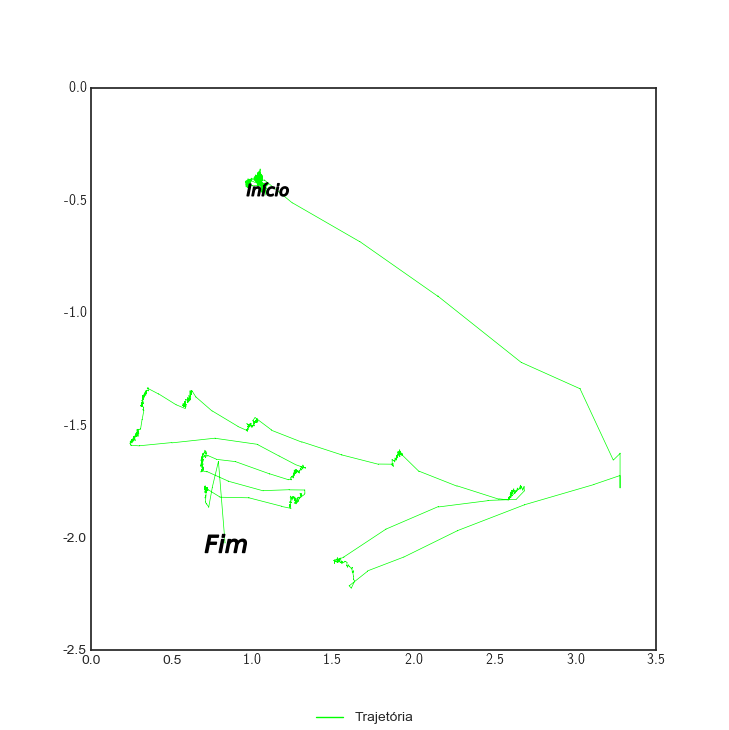
\includegraphics[scale=0.25]{imagens/trajetoria_dede.png}
                    \caption{Trajetória \textit{Dede}.}
                \end{center}
            \end{figure}
        \end{column}
        \begin{column}{0.48\textwidth}
            \begin{figure}[H]
                \begin{center}
                    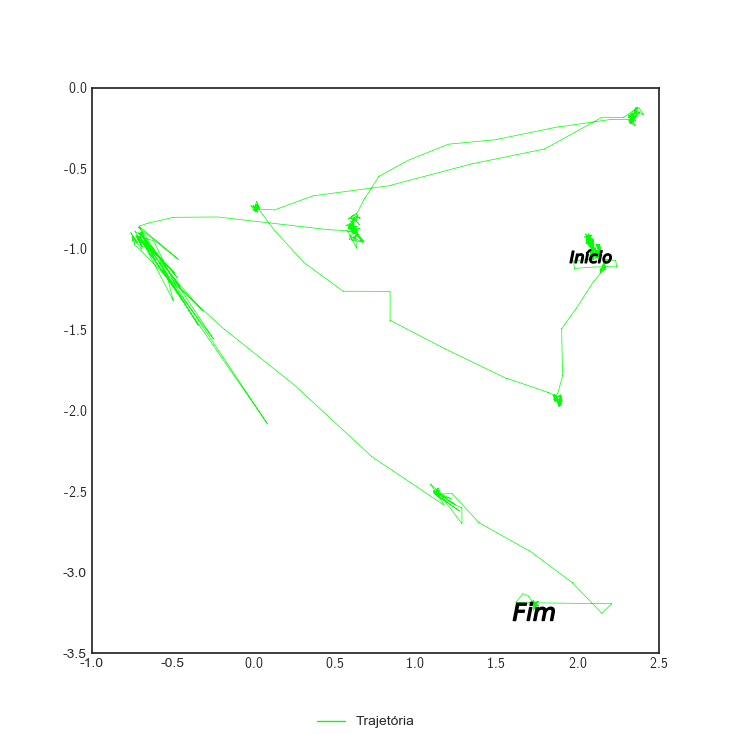
\includegraphics[scale=0.25]{imagens/trajetoria_juju.png}
                    \caption{Trajetória \textit{Juju}.}
                \end{center}
            \end{figure}
        \end{column}
    \end{columns}
\end{frame}

\begin{frame}{Dados Reais - Identificação de fixações e sacadas -  Métricas}
    \begin{table}[h]
        \centering
        \caption{Métricas utilizadas na avaliação com dados reais.}
        \label{tbl:metricas_rbfchain}
        \begin{tabularx}{\textwidth}{lX}
        \toprule
        Métrica  & Observação \\
        \midrule
        QP       &  \textbf{Quantidade de Pontos} analisados. \\
        AC       &  \textbf{Acurácia}.  \\
                 & Fração de fixações e sacadas identificadas corretamente. \\

        PR       &  \textbf{Precisão}.  \\
                 & Fração das fixações identificadas pelo algoritmo corretamente.  \\

        RE       &  \textbf{\textit{Recall}}.  \\
                 & Fração das fixações existentes (rotuladas) que também foram identificadas pelo algoritmo.  \\

        \bottomrule
        \end{tabularx}
        \end{table}
\end{frame}

\begin{frame}{Dados Reais - Identificação de fixações e sacadas -  Dede}
    \begin{columns}
        \begin{column}{0.48\textwidth}
            \begin{figure}[H]
                \begin{center}
                    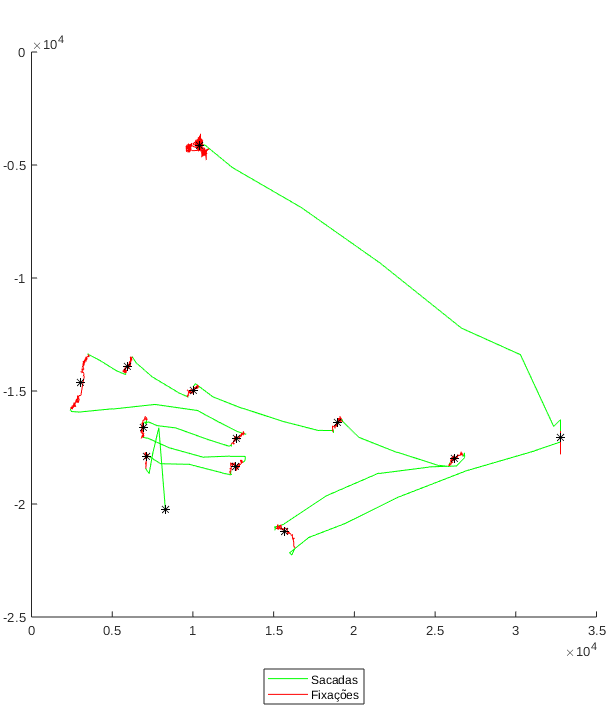
\includegraphics[scale=0.25]{imagens/dede_clusterfix.png}
                    \caption{ClusterFix - \textit{Dede}.}
                \end{center}
            \end{figure}
        \end{column}
        \begin{column}{0.48\textwidth}
            \begin{figure}[H]
                \begin{center}
                    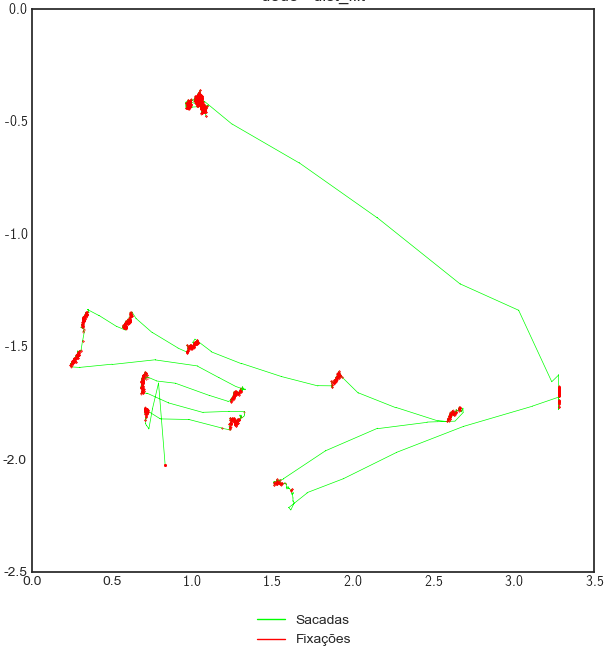
\includegraphics[scale=0.28]{imagens/dede_rbfchain.png}
                    \caption{RBFChain - \textit{Dede}.}
                \end{center}
            \end{figure}
        \end{column}
    \end{columns}
\end{frame}

\begin{frame}{Dados Reais - Identificação de fixações e sacadas -  Dede}
    \begin{table}[ht!]
        \centering
        \caption{Resultados para o conjunto de dados \textit{Dede}.}
        \label{tbl:dede}
        \begin{tabular}{llll}

        \toprule
        QT              & AC                     & PR                     & RE         \\
        \midrule
        $6.200$         & $0.87$                 & $0.98$                 & $0.88$      \\
        \bottomrule

        \end{tabular}
    \end{table}

    \begin{itemize}
        \item \alert{$87\%$} das fixações e sacadas identificadas pelo RBFChain tiveram a mesma classificação pelo ClusterFix.
        \item \alert{$98\%$} das fixações identificadas pelo RBFChain tiveram a mesma classificação pelo ClusterFix.
        \item \alert{$88\%$} das fixações identificadas pelo ClusterFix também foram identificadas pelo RBFChain.
    \end{itemize}
\end{frame}

\begin{frame}{Dados Reais - Identificação de fixações e sacadas -  Juju}
    \begin{columns}
        \begin{column}{0.48\textwidth}
            \begin{figure}[H]
                \begin{center}
                    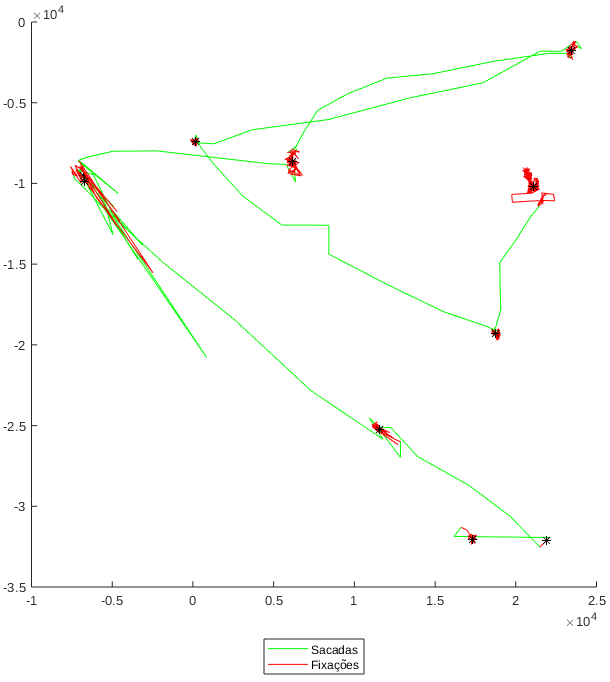
\includegraphics[scale=0.25]{imagens/juju_clusterfix.png}
                    \caption{ClusterFix - \textit{Juju}.}
                \end{center}
            \end{figure}
        \end{column}
        \begin{column}{0.48\textwidth}
            \begin{figure}[H]
                \begin{center}
                    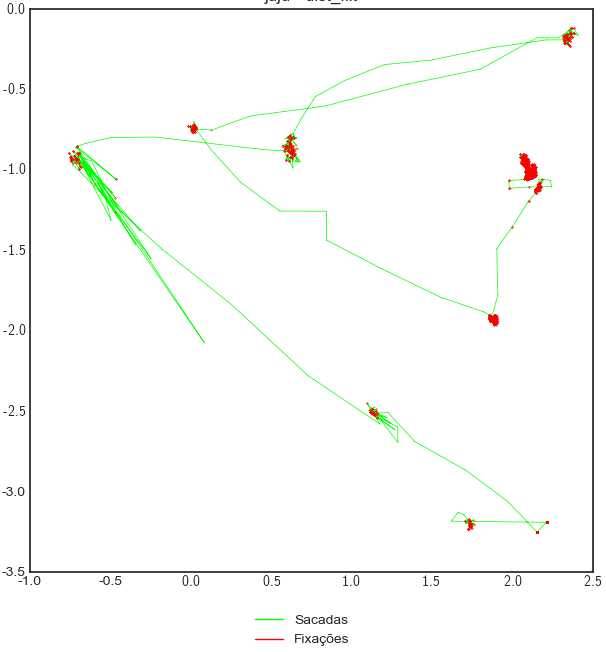
\includegraphics[scale=0.28]{imagens/juju_rbfchain.png}
                    \caption{RBFChain - \textit{Juju}.}
                \end{center}
            \end{figure}
        \end{column}
    \end{columns}
\end{frame}

\begin{frame}{Dados Reais - Identificação de fixações e sacadas -  Juju}
    \begin{table}[ht!]
        \centering
        \caption{Resultados para o conjunto de dados \textit{Juju}.}
        \label{tbl:juju}
        \begin{tabular}{llll}

        \toprule
        QT              & AC                     & PR                     & RE      \\
        \midrule
        $6.200$         & $0.82$                 & $0.98$                 & $0.83$      \\
        \bottomrule

        \end{tabular}
    \end{table}

    \begin{itemize}
        \item \alert{$82\%$} das fixações e sacadas identificadas pelo RBFChain tiveram a mesma classificação pelo ClusterFix.
        \item \alert{$98\%$} das fixações identificadas pelo RBFChain tiveram a mesma classificação pelo ClusterFix.
        \item \alert{$83\%$} das fixações identificadas pelo ClusterFix também foram identificadas pelo RBFChain.
    \end{itemize}
\end{frame}

\section{Novos experimentos e demonstração}

\end{document}
